\documentclass[tikz,border=2pt]{standalone}
\usepackage{amsmath,amssymb}
\usepackage{pgfplots}
\pgfplotsset{compat=1.18}
\usetikzlibrary{arrows.meta}
\begin{document}
% First-price auction, n = 3, theta = 0.9, rivals bid (2/3)theta: expected payoff
% E[u](b) = (0.9 - b)(1.5 b)^2 for b <= 2/3 and 0.9 - b above; maximum 0.243 at the
% equilibrium bid b = 0.6, deviations 0.5 -> 0.225 and 0.65 -> 0.238, bidding the value gives 0.
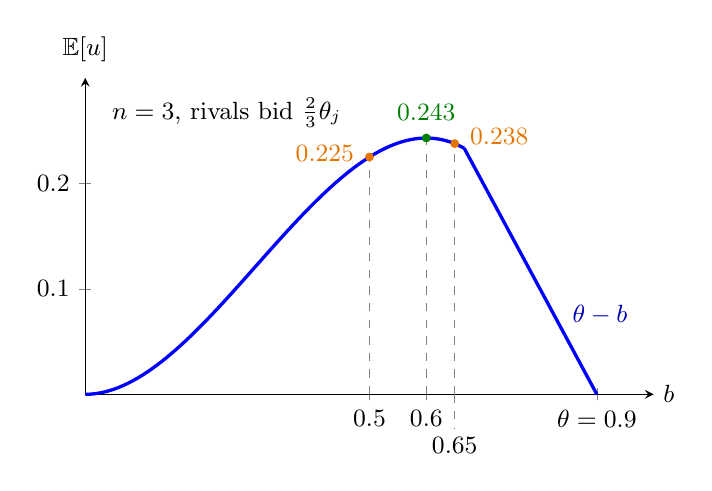
\begin{tikzpicture}[font=\small, >={Latex[length=2mm]}]
  \begin{axis}[
    width=8.8cm, height=5.6cm, axis lines=left,
    xmin=0, xmax=1.0, ymin=0, ymax=0.3,
    xtick={0.5,0.6,0.65,0.9}, xticklabels={$0.5$,$0.6$,,$\theta=0.9$},
    ytick={0.1,0.2}, yticklabel style={/pgf/number format/fixed},
    xlabel={$b$}, ylabel={$\mathbb E[u]$},
    xlabel style={anchor=west, at={(axis description cs:1,0)}},
    ylabel style={rotate=-90, anchor=south, at={(axis description cs:0,1.02)}},
    clip=false, every tick label/.append style={font=\small}]
    \addplot[blue, very thick, domain=0:2/3, samples=80] {(0.9-x)*(1.5*x)^2};
    \addplot[blue, very thick, domain=2/3:0.9] {0.9-x};
    % drop lines
    \draw[gray, thin, dashed] (axis cs:0.5,0) -- (axis cs:0.5,0.225);
    \draw[gray, thin, dashed] (axis cs:0.6,0) -- (axis cs:0.6,0.243);
    \draw[gray, thin, dashed] (axis cs:0.65,0) -- (axis cs:0.65,0.2377);
    % points
    \fill[orange!90!black] (axis cs:0.5,0.225) circle (1.6pt);
    \fill[orange!90!black] (axis cs:0.65,0.2377) circle (1.6pt);
    \fill[green!50!black] (axis cs:0.6,0.243) circle (1.6pt);
    \node[orange!90!black, anchor=east] at (axis cs:0.49,0.228) {$0.225$};
    \node[orange!90!black, anchor=west] at (axis cs:0.66,0.244) {$0.238$};
    \node[green!50!black, anchor=south] at (axis cs:0.6,0.25) {$0.243$};
    \draw[gray, thin, dashed] (axis cs:0.65,0) -- (axis cs:0.65,-0.032);
    \node[anchor=north] at (axis cs:0.65,-0.032) {$0.65$};
    % annotations
    \node[blue!70!black, anchor=west] at (axis cs:0.84,0.075) {$\theta-b$};
    \node[anchor=north west] at (axis cs:0.03,0.29) {$n=3$, rivals bid $\tfrac23\theta_j$};
  \end{axis}
\end{tikzpicture}
\end{document}
